%!TEX root = ../main.tex
%%%%%%%%%%%%%%%%%%%%%%%%%%%%%%%%%%
% Links:
% https://medium.com/@rsinghal757/kadanes-algorithm-dynamic-programming-how-and-why-does-it-work-3fd8849ed73d
% https://en.wikipedia.org/wiki/Maximum_subarray_problem
% https://www.geeksforgeeks.org/maximum-subarray-sum-using-divide-and-conquer-algorithm/
% https://www.geeksforgeeks.org/largest-sum-contiguous-subarray/ Difficulty: Medium Companies:
% Facebook paypal yahoo microsoft linkedin mazaon 
%%%%%%%%%%%%%%%%%%%%%%%%%%%%%%%%%%

\chapter{Largest sum in contiguous subarray}
\label{ch:max_sum_continguous_subarray}
\section*{Introduction}
When it comes to coding interview question, dynamic programming ones are among the most feared and challenging.
Among the most famous and iconic problem of this category is the \textit{Largest sum in contiguous subarray} problem which
is not only still nowadays asked frequently during interviews but has many real-life applications in science including, but not limited to, genomic sequence analysis (to identify certain protein sequences) and computer vision (to identify the brightest or darkest part of an
image). 

In this chapter we will investigate how to efficiently solve this problem and its most popular variations on the theme, starting from the inefficient brute-force solution which will serve as a starting point for our journey towards efficiency. This solution will then be improved by using the concept of avoiding duplicate calculation which is central to DP. 
Finally, we will study and develop an intuitive idea of what is considered to be the reference algorithm for this problem which allows us to solve this problem efficiently and elegantly.

\section{Problem statement}
\begin{exercise}
Write a function that finds the largest sum of a contiguous sub-array (containing at least one element) within an array $A$
of length $n$.

Formally, the task is to find two indices $ 0 \leq i \leq j < n$ s.t. the following sum is maximized:
\[
\sum_{x=i}^j   = A[x] = A[i] + A[i+1] + \ldots + A[j] 
\]

	\begin{example}
		\hfill \\
		Given $A=\{-2, -5, \underbrace{6, -2, -3, 1, 5}\text{}, -6\}$ then the answer is $7$ which can
		be obtained by summing all elements from index $2$ to $6$ i.e. $\sum_{2}^7 A[i] = 7$
	\end{example}

	\begin{example}
		\hfill \\
		Given $A=\{-2, 1, -3, \underbrace{4, -1, 2, 1}\text{}, -5, 4\}$ then the answer is $6$ which can
		be obtained by summing all elements from index $3$ to $6$ i.e. $\sum_{3}^6 A[i] = 6$
		
	\end{example}
\end{exercise}

\section{Clarification Questions}

\begin{QandA}
	\item Are the elements all positive or negative?
	\begin{answered}
		\textit{No, the input numbers can be either positive, or negative.}
	\end{answered}
	
	\item Is the array sorted?
	\begin{answered}
		\textit{No, the array is not sorted.}
	\end{answered}

	\item Is is guaranteed the final result fits an \inline{int}?
	\begin{answered}
		\textit{Yes, you should not worry about interger overflow.}
	\end{answered}
	
\end{QandA}

\section{Discussion}
\label{max_sum_continguous_subarray:sec:discussion}
A couple of important observations can be made after reading the problem statement:
\begin{itemize}
	\item If the array only contains non-negative numbers then the problem becomes trivial because the
	answer is the sum of the whole array.
	\item If, on the contrary, the array contains only  numbers lower or equal than zero, then the answer is
	coincides with the largest number in $A$ (if the constraint on the non-empty size of the sub-array is relaxed then, the answer in this case is always zero.).
	\item The answer is unique, but more than one sub-array might sum up to that value.
\end{itemize}

\subsection{Brute-force}
\label{sec:max_sum_continguous_subarray_bruteforce}
One way to tackle this problem is to look at the sum of all possible sub-arrays and return the largest.
The idea is that for all elements $A[i]$, the sum of \textbf{all} sub-arrays having it as starting
element can be calculated by as shown in Listing
\ref{list:max_sum_continguous_subarray_bruteforce}. The code uses enumerates all possible pairs of indices $i < j$, and for each of them calculates the sum of the elements of $A$ between $i$ and $j$. Among all of those sums, the largest is returned. 

This approach is correct but it is unnecessarily slow, and it has a time complexity of $O(n^3)$: there are $O(n^2)$ ordered pairs $(i,j)$ each identifying a sub-array, and calculating the sum of a single sub-array costs $O(n)$ (the call to \inline{std::accumulate}), for a grand total of $O(n^3)$. 
This is considered a poor solution because it is quite far off from the optimal linear time complexity solution that exists for this problem.

\lstinputlisting[language=c++, caption=Sample Caption,label=list:max_sum_continguous_subarray_bruteforce]{sources/max_sum_continguous_subarray/max_sum_continguous_subarray_solution1.cpp}


\subsection{Brute-force improved}
\label{max_sum_continguous_subarray:sec:bruteforce_improved}
The brute-force solution proposed in Section \ref{sec:max_sum_continguous_subarray_bruteforce} above can be
improved by avoiding to explicitly calculating the sum of a sub-array over and over again.
Given two indices $i$ and $j$ the corresponding sub-array sum can be obtained in constant time by using a pre-calculated
prefix sum (see Section \ref{sect:appendix:prefix_sum}) of the input array.
This allows for constant time computation of the sum of any sub-array in $A$. Given an array $Y$ containing the prefix sum for the
array $A$ then the sub-array sum between indices $i$ and $j$ is equal to: $Y[j]-Y[i-1]$ where $Y[-1] = 0$.

The code in Listing \ref{list:max_sum_continguous_subarray_bruteforce_improved} shows how this idea can be used to bring the time complexity of the the brute-force solution above (in Listing \ref{sec:max_sum_continguous_subarray_bruteforce}) down to $O(n^2)$. 
Notice how the call to \inline{std::accumulate} is substituted with a simple $O(1)$ operation on the prefix sum that is pre-calculated using the function \inline{prefix_sum} (which crucially runs in linear time).

\lstinputlisting[language=c++, caption=Brute-force solution using prefix-sum.,label=list:max_sum_continguous_subarray_bruteforce_improved]{sources/max_sum_continguous_subarray/max_sum_continguous_subarray_solution3.cpp}

Despite the dramatic improvement in time complexity obtained with this new solution, Listing
\ref{list:max_sum_continguous_subarray_bruteforce_improved} it is still considered a rather poor solution.
Storing the prefix sum costs linear space and  considering the the popularity of this interview question, during a real
interview a linear time and constant space solution is likely to be expected by the interviewer.

\subsection{Kadane's Algorithm}
\label{sec:kadane_algorithm}
There is an had-hoc algorithm named Kadane's algorithm that was developed to solve this problem efficiently by using a dynamic programming approach.
In its simplest form uses an additional array $B$ storing at each position $j$ the largest sum for a
sub-array ending (and including) at $A[j]$. Once $B$
is filled, the solution to the problem simply boils down to finding the maximum element in $B$. The idea above is coded 
in Listing \ref{list:max_sum_continguous_subarray_kadane_additional_space}.
\lstinputlisting[language=c++, caption=Linear space Kadane's algorithm.,label=list:max_sum_continguous_subarray_kadane_additional_space]{sources/max_sum_continguous_subarray/max_sum_continguous_subarray_solution2.cpp}

The core of this solution is in how $B$ is filled up. DP is used to calculate the value of each element $B[i]$ by reusing the information in the cell at index $i-1$. Clearly $B[0]$ cannot be anything different than $A[0]$ (there is only one sub-array ending at the first element of $A$), while for all the other locations we use \lstinline[columns=fixed]{std::max(A[i] , B[i-1]+A[i])} to decide the value of $B[i > 0 ]$. 
The function call to \inline{std::max} really means that the maximum sub-array sum ending at (and including) $A[i]$ comes from either:
\begin{enumerate}
	\item the sub-array starting and ending at index $i$ i.e. only containing $A[i]$, or
	\item extending the best sub-array ending at index $i-1$ by adding $A[i]$ to it. Notice that the sum of the
	best sub-array ending at $i-1$ is already computed and stored in $B[i-1]$. By doing so we are
	effectively avoiding a lot of re-computation, and this is the reason why Kadane's algorithm is
	so fast.
\end{enumerate}
If you think about it it make sense to construct $B$ this way. After all, when processing an element $A[i]$ you can either use it to extend a sub-array ending at index $i-1$ (and if you are going to extend one you are better off extending the one which gives you the largest sum up to that point) or start a new sub-array from the cell at position $i$. You choose one of the two option based on which choice lead to the largest value. 

Figure \ref{fig:median_sorted_array:kadane} shows an example of execution of this idea on the array $A=\{-2,-5,6,-2,-3,1,-10,4\}$ where it is depicted for each of the eight steps of the algorithm how the value for the corresponding cells of $B$ are calculated as well as which cells of $A$ contribute to it.

\begin{figure}
	\centering
	\begin{subfigure}[t]{0.48\textwidth}
		\centering
		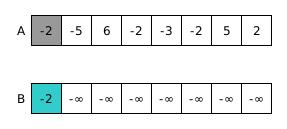
\includegraphics[width=\textwidth]{sources/max_sum_continguous_subarray/images/kadane1}
		\caption{$i=0$: $B[0]$ is equal to the first element of $A$}
		\label{fig:median_sorted_array:kadane0}
	\end{subfigure}
	\hfill
	\begin{subfigure}[t]{0.48\textwidth}
		\centering
		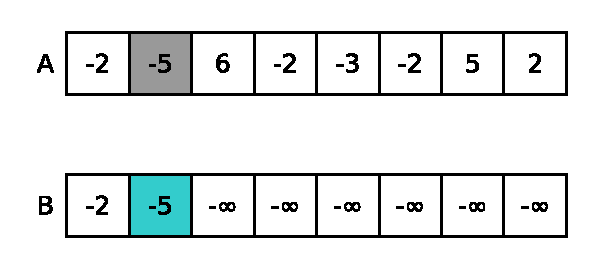
\includegraphics[width=\textwidth]{sources/max_sum_continguous_subarray/images/kadane2}
		\caption{$i=1$: $B[1]$ is equal to $A[1]$ only. $B[0]$ is negative and therefore $B[0]+A[1] < A[1]$.}
		\label{fig:median_sorted_array:kadane1}
	\end{subfigure}
	\hfill

	\begin{subfigure}[t]{0.48\textwidth}
		\centering
		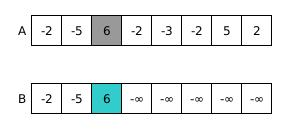
\includegraphics[width=\textwidth]{sources/max_sum_continguous_subarray/images/kadane3}
		\caption{$i=2$: $B[2]$ is equal to $A[2]$ only. $B[1]$ is negative and therefore $B[1]+A[2] < A[2]$.}
		\label{fig:median_sorted_array:kadane2}
	\end{subfigure}
	\hfill
	\begin{subfigure}[t]{0.48\textwidth}
		\centering
		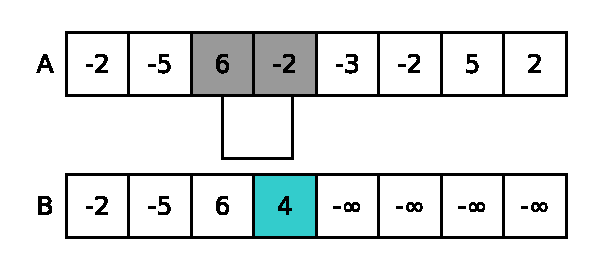
\includegraphics[width=\textwidth]{sources/max_sum_continguous_subarray/images/kadane4}
		\caption{$i=3$: $B[3]$ is equal to $A[2]+A[3]$. $B[2] > 0$ and therefore $B[2]+A[3] > A[3]$.}
		\label{fig:median_sorted_array:kadane3}
	\end{subfigure}
	\hfill

	\begin{subfigure}[t]{0.48\textwidth}
		\centering
		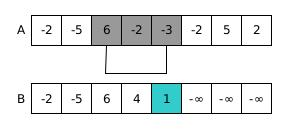
\includegraphics[width=\textwidth]{sources/max_sum_continguous_subarray/images/kadane5}
		\caption{$i=4$: $B[4]$ is equal to $A[3]+A[4]$. $B[3] > 0$ and therefore $B[3]+A[4] > A[3]$.}
		\label{fig:median_sorted_array:kadane4}
	\end{subfigure}
	\hfill
	\begin{subfigure}[t]{0.48\textwidth}
		\centering
		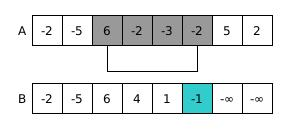
\includegraphics[width=\textwidth]{sources/max_sum_continguous_subarray/images/kadane6}
		\caption{$i=5$: $B[5]$ is equal to $A[4]+A[5]$. $B[4] > 0$ and therefore $B[4]+A[5] > A[5]$}
		\label{fig:median_sorted_array:kadane5}
	\end{subfigure}
	\hfill

	\begin{subfigure}[t]{0.48\textwidth}
		\centering
		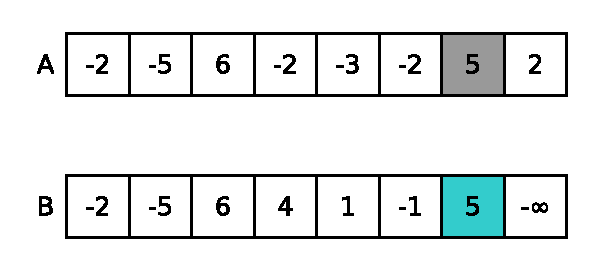
\includegraphics[width=\textwidth]{sources/max_sum_continguous_subarray/images/kadane7}
		\caption{ $i=6$: $B[6]$ is equal to $A[6]$ only. $B[5]$ is negative and therefore $B[5]+A[6] < A[6]$.}
		\label{fig:median_sorted_array:kadane6}
	\end{subfigure}
	\hfill
	\begin{subfigure}[t]{0.48\textwidth}
		\centering
		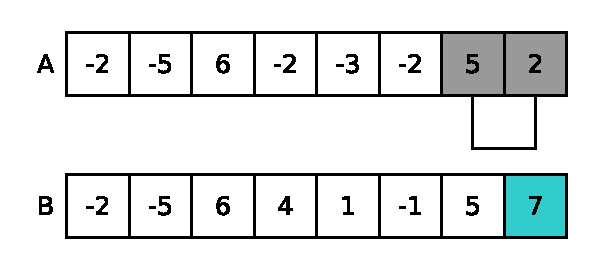
\includegraphics[width=\textwidth]{sources/max_sum_continguous_subarray/images/kadane8}
		\caption{$i=7$: $B[7]$ is equal to $A[6]+A[7]$. $B[6] > 0$ and therefore $B[6]+A[7] > A[7]$ }
		\label{fig:median_sorted_array:kadane7}
	\end{subfigure}
	\caption[Kadane's algorithm.]{This figure shows the array $B$ in the Kadane's algorithm is calculated. Gray cells are part of the sub-array that gives the value to the corrensponding cell in $B$ coloroued in cyan. }
	\label{fig:median_sorted_array:kadane}
\end{figure}


\subsubsection{Linear time and constant space Kadane's algoritm}
But, is the additional space used by $B$ really necessary? A closer look at the implementation in
Listing \ref{list:max_sum_continguous_subarray_kadane_additional_space} provides the answer which
is, no. In-fact every value of $B$ is only used \textbf{once}, and then ignored for the rest of the execution.
Thus the algorithm can be modified to take advantage of this fact so it only uses a single variable to store the latest calculated
value of $B$ i.e. the value for the index $i-1$ as shown in Listing
\ref{list:max_sum_continguous_subarray_kadane}

\lstinputlisting[language=c++, caption=Constant space and linear time Kadane's algorithm,label=list:max_sum_continguous_subarray_kadane]{sources/max_sum_continguous_subarray/max_sum_continguous_subarray_solution4.cpp}

Note how the variable \texttt{max\_ending\_here} is doing the job that the variable \texttt{B[i-1]}
was doing in Listing \ref{list:max_sum_continguous_subarray_kadane_additional_space} and also how
the final answer is the maximum among all values taken by \texttt{max\_ending\_here}.

The complexity of this approach is $O(n)$ in time and $O(1)$ in space, and very likely is the sort
of complexity the interviewer expects.

\section{Common Variations}
\subsection{Minium sum contiguous sub-array}
A very common variation of this problem is to find the smallest sum instead of the largest. This
variation is very quickly solved by just changing the the way the variables in Listing \ref{list:max_sum_continguous_subarray_kadane}
\texttt{min\_ending\_here} (the variable is named \textbf{min} instead of max so to reflect the nature of the
problem) and \texttt{ans} are updated. Since the minimum is to be returned then they should be
updated using \lstinline[columns=fixed]{min_ending_here = std::min(A[i] , max_ending_here+A[i]);}
and \lstinline[columns=fixed]{std::min(ans, in_ending_here);}, respectively.  

\subsection{Longest positive/negative contiguous sub-array}
Another common variation of the max/min sum contiguous subarray is to find the longest subarray only
made of positive or negative numbers. The same core idea used for the other variant can be used here
as well. At each iteration $i$ the variable \texttt{longest\_ending\_here} represents the longest
positive subarray up to that iteration and including the element $A[i]$ and can be updated as
follows: \lstinline[columns=fixed]{longest_ending_here = A[i] >= 0 ? longest_ending_here+1 : 0;}.